\section{Introduction}

A \textbf{database} is a collection of related data (=known facts that can be recorded and have implicit meaning). There is a focus on information (interpretation of what is stored), not only on storage.\\

\textbf{Properties:}
\begin{itemize}
    \item Represents some aspects of the world (=\textbf{miniworld} or \textbf{Universe of Discourse}). Changes to the miniworld are reflected in the database. It is all about what information needs to be captured.
    \item Logically coherent collection of data with some meaning.
    \item It is designed, built and populated with data for a \textbf{specific purpose}. It has an intended group of users and some preconceived applications.
\end{itemize}

All those properties make the databases a way of storing data with higher specifications.\\

A \textbf{DataBase Management System} is a computerized system that enables users to create and maintain a database. It is a general purpose software system that facilitates the processes of defining, constructing, manipulating and sharing databases among various users and applications. It is also used to protect and maintain the database.\\

The database base and the DBMS software together are called a \textbf{database system} (cfr. figure \ref{fig:databaseSystem}).

\begin{figure}[!h]
    \centering
    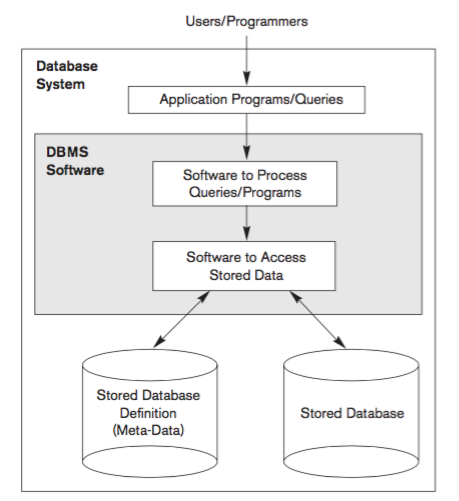
\includegraphics[scale=0.4]{chap1-1.png}
    \caption{A simplified database system environment}
    \label{fig:databaseSystem}
\end{figure}

\section{Characteristics of the Database Approach}

In \textbf{file processing}, each user defines and implements the files needed for a specific software application as part of programming the application. There is \textbf{redundancy} because each user maintains separate files. Moreover, if someone writes to a file and then shutdowns the system, there is no guarantee that the data have been written.\\

In the \textbf{database approach}, a single repository maintains data that is defined once and then can be accessed by various users.\\

\textbf{Main differences between databases and files:}
\begin{itemize}
    \item \textbf{Self-describing} nature of a database system
    \item \textbf{Insulation} between programs and data, and data abstraction
    \item Support of multiple \textbf{views} of data
    \item Sharing of data and \textbf{multi-user} transaction processing
\end{itemize}

\subsection{Self-describing nature}
The database system contains a complete definition of the database structure and constraints (its own model). It is stored in the DBMS catalog and is called the \textbf{meta-data}. The DBMS catalog also contains information about the structure of each file, the type and storage format of each data item and various constraints on the data. \textbf{NOSQL} systems do not require meta-data because they contain self-describing data that include the names and values together in one file.\\

File processing software can only access files with a specific structure. Whereas DBMS can access diverse databases by extracting the database definitions from the catalog. Moreover, the model of data is hardcoded. So there might be problems if the program is lost.\\

In files, there is a tight coupling between programs and physical data organization. If one of them changes, the other one must change too. The files and the data structure are \textbf{coupled}, it is bad.\\

\textbf{Coupling} happens when two things are strongly dependent. If one of them is broken, the system formed by those two things is broken too.

\subsection{Insulation between programs and data, and data abstraction}

The structure of data files is stored in the DBMS catalog, separately from the access programs. So a change to the structure does not always require to rewrite the program. It is called \textbf{program-data independence}. It is important to be able to change things (add a field, reorganize file, ..) without breaking everything (\textbf{management of changes}).\\

In some database systems, users can define \textbf{operations} (functions) that can be called regardless of how they are implemented. It is called \textbf{program-operation independence}.\\

Those two characteristics are allowed thanks to \textbf{data abstraction}. The DBMS provides \textbf{conceptual representation} without many details of how the data is stored or how the operations are implemented. A \textbf{data model} is a kind of data abstraction that is used to provide this conceptual representation.\\

The \textbf{conceptual schema} (neutral view) is between the external and the internal schemes.

\begin{figure}[!h]
    \centering
    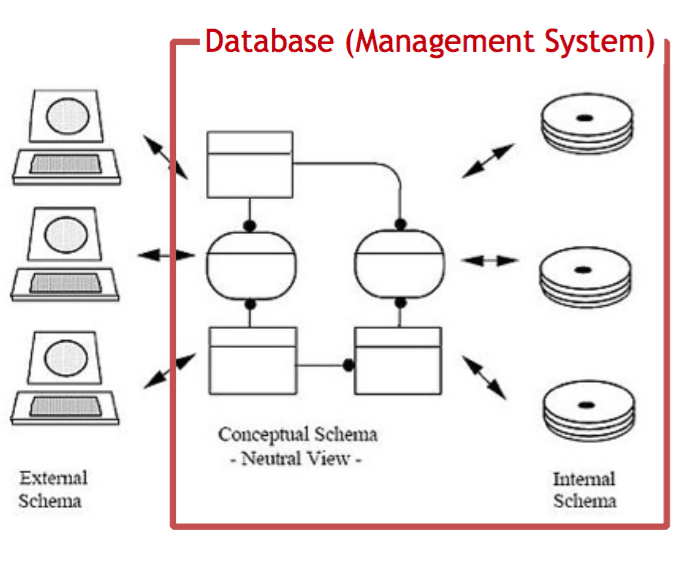
\includegraphics[scale=0.4]{chap1-2.png}
    \caption{Three schema architecture}
    \label{fig:architecture-1}
\end{figure}

Changes of data structures at the physical level (internal schema: disk) should be kept transparent at the logical level (external schema: user, programs).

\subsection{Support of Multiple Views of the Data}
A database has many types of users, each of whom may require a different perspective or view of the database. It can be a subset of the database or virtual data that is not stored.\\

Files have low level from an information standpoint.

\subsection{Sharing of Data and Multiuser Transaction Processing}

A multi-users DBMS must allow several users to access the database at the same time. There must be a \textbf{concurrency control} software to ensure that several users trying to update the same data do it in a controlled manner. These types of applications are often called \textbf{online transactions processing} (OLTP).\\

A relational database has a declarative query language. It describes what we want to do, not how (and it doesn't describe the control flow either).

A \textbf{transaction} is an executing program or process that includes one or more database accesses (reading or updating). If a transaction is executed completely, it is supposed to execute a logically correct database access.\\

It must also respect the \textbf{ACID} specification. They guarantee that concurrent databases transactions are processed reliably:\\

\begin{itemize}
    \item \textbf{Atomicity} : Either all database operations in a transaction are executed or none are.
    \item \textbf{Consistency}: Gives the correct answer. There are rules (invariants) that must always be true. For example, the value of $x$ must be in the interval [4,100]. It ensures that the database always goes from one valid state to another.
    \item \textbf{Isolation} Each transaction appears to execute in isolation from other transactions. Guarantee that even if many users use the database either one user see the other transactions because they are finished or he doesn't see them. The partial effects are invisible before the commit.
    \item \textbf{Durable}: If the system tells us that some data is stored after a commit, we can reboot it and it will still be there.
\end{itemize}

With files, it is hard to manage concurrent updates and failures. For example if several users want to read or write at the same time or if the system gets unplugged.

\section{Advantages of Using the DBMS Approach}
\subsection{Controlling redundancy}

Redundancy can cause several problems:

\begin{itemize}
    \item \textbf{Duplication of effort}: A single logical update must be performed several times (once for each file where this data is recorded).
    \item \textbf{Storage space wasted}
    \item \textbf{Data may become inconsistent}: it may happen if an update is not applied to all the files or different data can be written
\end{itemize}

\textbf{Data normalization} ensures consistency and saves storage space. However \textbf{controlled redundancy} can be used to improve performances (for example storing the student's id, course's id and grade in one summary table). The redundancy can be controlled with constraints and foreign keys to avoid inconsistency.

\subsection{Restricting unauthorized access}

Restrict the data that an user can access or the operations that he can perform. Users and user groups have accounts protected by passwords. The DBMS should provide a security and authorization subsystem to create accounts and specify restrictions. 

\subsection{Providing Persistent Storage for Program Objects}

Databases can be used to provide \textbf{persistent storage} for program objects and data structures. This is one of the main reasons for \textbf{object-oriented database systems}. It is easier and safer than storing the objects in the file with a specific format and then having to parse it.

\subsection{Providing Storage Structures and Search Techniques for Efficient Query Processing}

Database systems must be able to efficiently execute queries and updates. The DBMS must provide specialized data structures and search techniques to speed up the search on disk. Auxiliary files called \textbf{indexes} are used for this purpose. The DBMS often has a \textbf{buffering} or \textbf{caching} module.\\

The \textbf{query processing and optimization} module is responsible for choosing an efficient query execution plan for each query. The choice of which index to create and maintain is part of the physical database design and tuning.

\subsection{Providing Backup and Recovery}

A DBMS must provide facilities for recovering from hardware or software failures. For example, if the computer system fails in the middle of an update transaction, the recovery subsystem is responsible for making sure that the database is restored to the state it was in before the transaction started executing.

\subsection{Providing Multiple User Interfaces}

A DBMS should provide a variety of user interfaces (apps for mobile users, query languages, programming interfaces ...).

\subsection{Representing Complex Relationships among Data}

A DBMS must be able to represent complex relationships among data, to define new relationships as they arise and to retrieve and update related data easily and efficiently. 

\subsection{Enforcing integrity constraints}

Most databases have \textbf{integrity constraints} that must hold for the data. A DBMS should provide capabilities for defining and enforcing these constraints. 

\textbf{Examples of integrity constraints}:

\begin{itemize}
    \item Data type for each data item (ex. name must be a string of no more than 30 letters)
    \item Referential integrity constraint (foreign key)
    \item Key or uniqueness constraint
\end{itemize}

Constraints that aren't checked automatically and that must be checked by update programs or at the time of data entry are called \textbf{business rules}. Rules that pertain to a specific data model are called \textbf{inherent rules}.

\subsection{Permitting Inferencing and Actions Using Rules and Triggers}

\textbf{Deductive database systems} provides capabilities for defining deduction rules for inferencing new information from the stored facts. For example there might be rules to determine all students on probation. \\

A \textbf{trigger} is a form of rule activated by updates to the table, which results in performing some additional operations to some other tables.\\

\textbf{Stored procedures} are more involved procedures to enforce rules. They are part of the overall database definition and are invoked when some conditions are met. \\

\textbf{Active database systems} provide active rules that can automatically initiate actions when certain events and conditions occur.

\subsection{Additional implications of using the database approach}

\begin{itemize}
    \item \textbf{Potential for enforcing standards}: names and formats of data elements, display formats, reports structures, terminology ...
    \item \textbf{Reduced application development time}: once a database is up and running, less time is required to create new applications using DBMS facilities.
    \item \textbf{Flexibility}: it may be necessary to change the structure of a database as requirements change. Modern DBMSs allow certain types of evolutionary changes to the structure of the database without affecting the stored data and the existing application programs.
    \item \textbf{Availability of up-to-date information}: a DBMS makes the database available to all users. Every user can see the updates immediately. 
    \item \textbf{Economies of scale} : the DBMS approach permits consolidation of data and applications
\end{itemize}

\section{A brief history of database applications}

One of the main problems with early database systems was the intermixing of conceptual relationships with the physical storage and placement on the disk. They did not provide enough \textbf{data abstraction} and \textbf{program-data independence} capacities. New queries that required a different storage organization for efficient processing where difficult to implement. \\

\textbf{Relational databases} were originally proposed to separate the physical storage of data from its conceptual representation and to provide a mathematical foundation for data representation and querying. They use relations that are represented by tables. A relation is only used to give meaning to the stored data.\\

The relational model says nothing about:\\

\begin{itemize}
    \item How relations are stored
    \item How data is to be distributed over nodes/servers
    \item What data types are available
    \item How tuples are ordered, indexed
\end{itemize}

\section{When not to use a DBMS}

\textbf{Overhead costs of using a DBMS}:

\begin{itemize}
    \item High initial investment in hardware, software and training
    \item Generality that it provides for defining and processing data
    \item Overhead for providing security, concurrency control, recovery and integrity functions
\end{itemize}

It might not be desirable to use a DBMS in the following situations:\\

\begin{itemize}
    \item Simple, well-defined database applications that are not expected to change at all
    \item Stringent, real-time requirements for some application programs that may not be met because of DBMS overhead
    \item Embedded systems with limited storage capacity, where a general-purpose DBMS would not fit
    \item No multiple-user access to data
\end{itemize}

\section{Main causes for NoSQL and NewSQL}

\begin{itemize}
    \item \textbf{Big data}: too much data for relational implementation to handle the load
    \item \textbf{Relational pack overused}: many software simply require storage, not all software are multi-user and sometimes we don't need to have the ACID properties.
    \item \textbf{Requires upfront thinking}: the current motto is \textbf{do and then think}
    \item \textbf{SQL has many flaws}: for example lack of user-defined data types
    \item \textbf{Data independence}: it can be achieved by other means when the data layer offers a low-level quality of service.
    \item The relational model is about working with \textbf{high-level abstractions} (for weak coupling, long-term maintenance, meeting the needs of every user even the ones we don't know yet). No one is favoured regarding data access. It is not compatible with the way most new businesses want to work
\end{itemize}

\section{Summary}

The keys messages are the following:\\

\begin{itemize}
    \item \textbf{Database definition}: focus on information, not only storage
    \item \textbf{Data independence}: weak coupling for easier maintenance
    \item \textbf{High-level specification}: behavioral guarantees for meeting requirements
    \item \textbf{Declarative vs procedurale}: Information aims at being queried
\end{itemize}

\textbf{\textcolor{red}{Examples of exam question}}:
\begin{itemize}
    \item Give two main ideas for the database (example: decoupling and ACID)
    \item Why were databases invented with hard disk (because they provide random accesses, on tapes there were only sequential accesses).
    \item Give 5 examples of physical changes that don't affect the external schema 
    \begin{itemize}
        \item Encoding
        \item Different file organization or storage structures
        \item Storage devices (hard-disk or SSD)
        \item Indexing strategy (hash index, B-tree ..)
        \item Switching from one access method to another
        \item Exact location of data on disk
        \item Compression
        \item Splitting
        \item Merging of records
    \end{itemize}

\end{itemize}